\chapter{Descrizione}


Deel implementa le funzionalità più comuni ricercate in un servizio di
hosting  quali l'upload di file di varie dimensioni, il
download, lo sharing, l'organizzazione gerarchica in cartelle e il
versionamento automatico dei file caricati sul sistema, nonchè la gestione del
proprio account.

\subsection{Struttura}


%% Da vedere
% applicazione ? stata sviluppata utilizzando il pattern di
% programmazione MVC. Tuttavia non tutta la logica riguardante la
% componente dei controller viene implementata lato server ma,
% attraverso tecnologie di chiamate asincrone (AJAX), anche lato
% client. 

L'applicazione è stata suddivisa in moduli interdipendenti tra loro,
ognuno dei quali si occupa di precise funzionalità chiave. Ogni modulo
espone agli altri moduli  solo
la propria interfaccia, mantenendo privata l'implementazione, così da aumentare
la possibilità di riutilizzo e manutenzione del codice. 
I principali moduli sono mostrati nella figura \ref{arc}. 

\begin{figure}
\center
  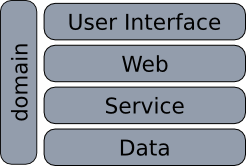
\includegraphics{architecture}
\caption{}
  \label{arc}
\end{figure}


\subsection{Domain}
Le classi che fanno parte del dominio rappresentano la  modellazione del
problema svincolata dalle logiche di accesso ai dati, persistenza,
navigazione ecc. Le classi sono strutturate come semplici POJO (plain
old java object) così da non dipendere da nessun tipo di framework
particolare. Le classi si trovano nel package java org.deel.domain.

\subsection{Data layer}

Si occupa della persistenza dei dati, e di fornire un mapping
consistente tra i dati permanenti e i dati manipolati in memoria
dall'applicazione. Per salvare i metadati relativi ai file ed i dati
relativi agli utenti è stato utilizzato un DBMS, in particolare
MySQL. I file veri e propri vengono salvati utilizzando le
funzionalità di accesso al filesystem del sistema operativo. Per
consentire il mapping tra oggetti del database e oggetti utilizzati
dal sistema sono state utilizzate le funzionalità del framework
Hibernate.
Lo schema E-R dell' applicazione è definito nella
figura \ref{ER}. 

\begin{figure}
  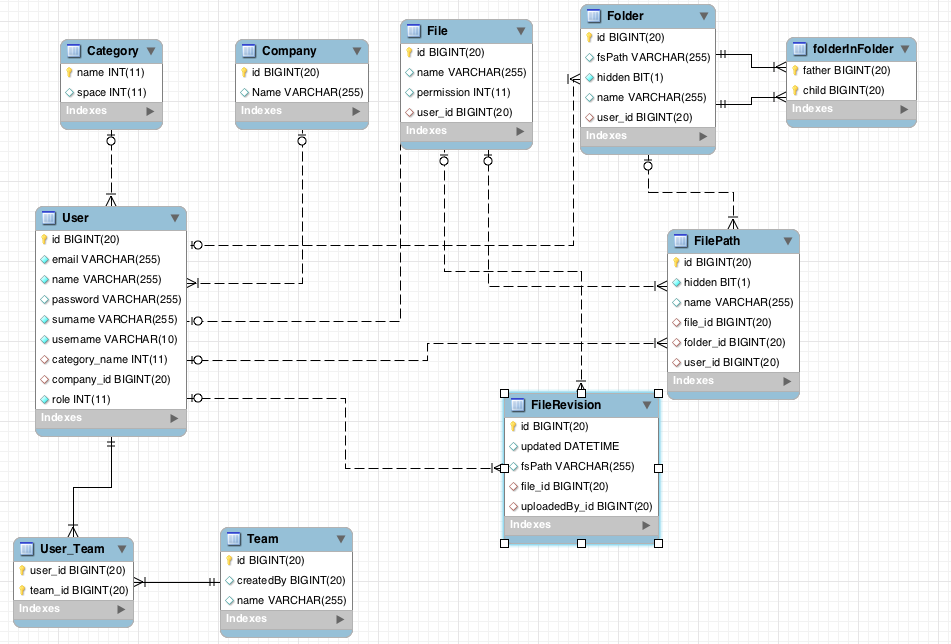
\includegraphics[scale=0.4]{er}
  \caption{}
  \label{ER}
\end{figure}


Ogni utente ha i propri file uplodati organizzati attraverso una
struttura di tipo file-system, dove file e cartelle sono organizzati
in una struttura ad albero. Questa struttura è stata implementata nel
database attraverso le tabelle filePath e folder, separando quindi i
nodi che non possono avere discendenti (i FilePaths) dal resto
dell'albero.

Ad ogni filePath è associato un File. Più filePath possono essere
associati al medesimo File. In questo modo la condivisione avviene
grazie a diversi FilePath indipendenti, appartenenti a utenti diversi, ma
che hanno associato il medesimo File. Ogni File avrà poi la propria
lista di revisioni, anch'esse condivise.

Per la configurazione di Hibernate sono state utilizzate
annotazioni sulle classi del layer Domain.  Le relazioni tra le entità
sono state mappate in modo bidirezionale, così da consentire la
navigazione delle relazioni tra entità senza dover codificare
istruzioni sql manualmente. 

La strategia di caricamento scelta è stata Lazy, per evitare
catastrofici caricamenti ricorsivi di tutto il Database in memoria e
eseguire query sql solo quando ve ne sia effettivamente bisogno.
Hibernate e' stato integrato nell'applicazione attraverso la
configurazione di due bean di spring, in particolare sessionFactory e
TransactionManager. Il sessionFactory provede ad istanziare una
sessionFactory di Hibernate e settarla come proprietà delle classi che
la utilizzeranno per rendere persistenti nel db gli oggetti del
dominio. Il transaction manager consente invece di definire i
boundaries delle transazioni in modo dichiarativo, tramite l'utilizzo
dell'annotazione @Transactional.  In questo modo il codice è
svincolato dal dover far iniziare, committare e rollbackare la
transazione in modo esplicito. Infine per la propragazione delle operazioni sul DB abbiamo
deciso, tranne per particolari casi, di non propagare nessuna
operazione, così da avere maggiore controllo su inserimenti e
rimozioni a livello di business logic.




\subsection{Service layer}

Il service layer si occupa di implementare i principali casi d'uso
dell' applicazione, manipolando sia oggetti del domain sia interagendo
con il data layer.  Il layer Service è stato progettato in modo tale
di aver associato un caso d'uso per ogni metodo, rappresentando l'area
di responsabilità di una Unit Of Work, che deve quindi preservare, tra
le altre, la proprietà di atomicità. Questi infatti sono i metodi che
sono stati annotati come @Transactional, in modo che il transaction
manager di Spring inizi la transazione al momento della chiamata del
metodo, ``committi'' al suo completamento o faccia il rollback in caso
di errori.Il service layer, come il layer web, utilizza la
dependency injection del framework Spring. In questo modo
l'istanziazione degli oggetti di cui questo layer necessita (ad
es. gli oggetti con le funzionalità di persistenza dei dati presenti
nel data layer) avviene in maniera automatica e il codice non dipende
da essa.

\subsubsection{Consistenza tra Database e Filesystem}
La gestione delle transazioni è dichiarativa. Un errore, e quindi il
lancio di un eccezione, da parte delle operazioni sul filesystem
causerà quindi il rollback della transazione sul database. Se è invece
è la transazione a non poter essere ``committata'' deve essere
previsto un meccanismo per mantenere la consistenza tra Database e
Filesystem. Nella nostra applicazione questa funzionalità è stata
implementata tramite la \emph{programmazione orientata agli aspetti}.
In particolare è stato utilizzato il modulo \emph{Spring AOP} e sono
stati inseriti gli opportuni \emph{advice} affinchè l'aspetto tenga
traccia delle modifiche effettuate sul filesystem e nel caso avvenga
un rollback da parte della transazioni ripristini lo stato dello
stesso. Per quanto riguarda la concorrenza, le operazioni effettuate
da un singolo utente sono seriali, ogni utente ha la propria area e
quindi non vi possono essere errori dovuti ad un accesso concorrente
allo stesso file o cartella.

\subsection{Web Layer}

Il web layer si occupa della logica di navigazione e della
gestione della sicurezza dell'applicazione. 

Per l'implementazione della sicurezza (acesso e autenticazione) è
stato utilizzato il modulo Spring Security, che tramite filtri serlvet
permette una acesso selettivo e autenticato al sistema. Le password
vengono salvate nel db utilizzando l'implementazione java di
\emph{BCrypt} (le password vengono hashate, saltate e strechate). Sono
stati implementati due diversi role (USER e ADMIN), in modo da avere
un'area per la gestione dell'applicazione accessibile sono agli utenti
amministratore.


Per quanto riguarda la navigazione sono state utilizzate le
funzionalità offerte dal modulo Spring MVC, funzionante su un servlet
container (ad es. tomcat). Quando una richiesta arriva
all'applicazione essa viene mappata all'opportuno
\emph{Controller}. Il mapping viene definito tramite annotazioni sul
codice java. Il Controller, nel caso di una richiesta HTML, si occupa
di validare l'input (anche questo viene definito grazie ad
annotazioni), di chiamare gli opportuni metodi sul layer service, di
esporre i dati del modello e di indicare il nome di una vista da
visualizzare all'utente. Se invece la richiesta è ti tipo JSON, dopo
la validazione dell'input e le interazione con il layer service il
controller ritorna le informazioni richieste al client sotto forma di
oggetto JSON. In questo modo abbiamo potuto delegare parte della
logica riguardate la User Interface sul lato client, fornendo da una
parte una migliore e più reattiva esperienza utente, dall'altra
diminuendo in qualche modo il carico di lavoro sul lato server.

\subsection{User Interface}

E' il layer più vicino all'utente e l'unico con cui interagisce
direttamente. Una volta che il controller indica il nome il nome di
una vista e i dati da esporre, in modo totalmente configurabile questo
nome viene mappato ad una tecnologia di visualizzazione. In questo
modo è facile aggiungere nuove tecnologie di rendering senza
modificare il layer web. Nel nostro caso abbiamo utilizato i tag JSTL
utilizzati per renderizzare i contenuti da esporre in una pagina html
finale.  Per migliorare l'esperienza utente parte di questa logica è
stata portata sul lato client. Del codice javascript in questo caso
esegue le richieste in modo asincrono al server grazie ad AJAX, e,
tramite un meccanismo di callback, aggiorna dinamicamente il contenuto
della pagina. Si è utilizzato jQuery come libreria.


\chapter{Sviluppo}

\subsection{Ambiente, IDE e testing}

Come ambiente di sviluppo sono stati utilizzati diversi tool e
strategie.  Si è proceduto nello sviluppo del software anche seguendo
una metodologia di tipo Test Driven. Si è cioè proceduro prima alla
creazione di unit test per la funzione da implementare per poi solo in
un secondo momento scrivere la reale implementazione. L'utilizzo della
dependecy injection insieme a l'utilizzo di tool per lo unit testing
come \emph{JUnit}, \emph{Spring Test Framework} e \emph{mockito} hanno consentito di
scrivere test piccoli, mirati, utili e facili da mettere in piedi.

Come IDE si è scelto di utilizzare \emph{Eclipse}, come
tool di building e per la gestione delle dipendenze \emph{Maven}.

\subsection{Caso d'uso d'esempio}

In figura \ref{upload} è mostrato il diagramma di sequenza
semplificato del caso d'uso riguardante l'upload di un file da parte
dell'utente. E' possibile fare l'upload di un file trascinandolo
direttamente dal Sistema. Una volta droppato il file, parte una
richiesta asincrona fatta dal client al server. 



\begin{figure}
  
\includegraphics[scale=0.4]{upload}
  \caption{}
  \label{upload}
\end{figure}

\chapter{Conclusioni}

L'utilizzo dei framework Spring e Hibernate ci ha consentito di
utilizzare in poco tempo pattern essenziali nella programmazione di
applicazioni enterprise quali data mapping, lazy loading, Inversion of
Control, Unit of Work e altri. Si è cercato per quanto possibile di
rendere il codice indipendente da tecnologie in particolare,
utilizzando notazioni JPA dove possibile e non inserendo caratteriste
dipendendi dal DBMS sottostante. Un approccio modulare che favorisce
la riusabilità e la manutenzione del codice.

%%% Local Variables: 
%%% mode: latex
%%% TeX-master: "relazione"
%%% End: 
